
\documentclass{article}
\usepackage[final]{neurips_2019}

\makeatletter
\renewcommand{\@noticestring}{Deep Learning, Sommer 2019, Universiteit van Amsterdam}
\makeatother

\usepackage{comment}
\usepackage{amsmath}
\usepackage{amssymb}
\usepackage{multirow}
\usepackage{verbatim}

\usepackage{hyperref}
\usepackage{algorithm}
\usepackage{algpseudocode}
\usepackage{nicefrac}
\usepackage{graphicx}
\usepackage{caption}
\usepackage{subcaption}
\usepackage{dsfont}
\usepackage{bm}
\usepackage[utf8]{inputenc}
\usepackage[T1]{fontenc}
\usepackage{url}
\usepackage{booktabs}
\usepackage{microtype}
\usepackage{tabularx}

% Matrices
\newcommand\bM[1]{\ensuremath{\begin{bmatrix}#1\end{bmatrix}}}
\newcommand\vM[1]{\ensuremath{\begin{vmatrix}#1\end{vmatrix}}}
\newcommand\BM[1]{\ensuremath{\begin{Bmatrix}#1\end{Bmatrix}}}

% operators and fractions
\newcommand\·{\ensuremath{\cdot}}
\newcommand\…{\ensuremath{\ldots}}
\newcommand\p{\ensuremath{\partial}}
\renewcommand\t{\ensuremath{\times}}
\newcommand{\LRA}{\ensuremath{\Leftrightarrow}}
\DeclareMathOperator*{\argmax}{arg\,max}
\DeclareMathOperator*{\argmin}{arg\,min}
\DeclareMathOperator{\adj}{Adj}
\DeclareMathOperator{\Tr}{Tr}
\DeclareMathOperator{\Dir}{Dir}
\DeclareMathOperator{\sgn}{sgn}

\newcommand\f[2]{\ensuremath{\frac{#1}{#2}}}
\newcommand\nf[2]{\ensuremath{\nicefrac{#1}{#2}}}
\newcommand\pf[2]{\ensuremath{\frac{\partial {#1}}{\partial {#2}}}}

% Typesetting and symbols
\newcommand*{\B}[1]{\ifmmode\bm{#1}\else\textbf{#1}\fi}
\newcommand*{\I}[1]{\ifmmode\mathit{#1}\else\textit{#1}\fi}
\newcommand\1{\ensuremath{\mathds{1}}}
\newcommand\E{\ensuremath{\mathds{E}}}
\newcommand\R{\ensuremath{\mathds{R}}}
\newcommand\N{\ensuremath{\mathcal{N}}}
\newcommand\w{\ensuremath{\mathbf{w}}}

\renewcommand{\thesubsubsection}{\thesubsection.\alph{subsubsection}}

\title{Assignment 1. MLPs, CNNs and Backpropagation}
\author{%
  Maurice Frank\\
  11650656\\
  \href{mailto:maurice.frank@posteo.de}{maurice.frank@posteo.de} \\
}

\begin{document}
\maketitle
\section{MLP backprop}
\subsection{}
\subsubsection{}
\begin{align*}
  \tag{$\pf{\B{x}^{(N)}}{\B{L}}$}
  \pf{\B{L}}{x_i^{(N)}}
  &= -\pf{}{x_i^{(N)}}\sum_i t_i \log x_i^{(N)}\\
  &= -t_i\·\f{1}{x_i^{(N)}}\\
  &\LRA\\
  \pf{\B{L}}{\B{x}^{(N)}}
  &= -[\hdots \f{t_i}{x_i^{(N)}}\hdots]\\
  &\in\R^{d_N}
\end{align*}

\begin{align*}
  \tag{$\pf{\B{x}^{(N)}}{\tilde{\B{x}}^{(N)}}$}
  \pf{x_i^{(N)}}{\tilde{x_j}^{(N)}}
  &= \pf{}{\tilde{x}_j^{(N)}}\f{\exp{\tilde{x}_i^{(N)}}}{\sum_k \exp{\tilde{\B{x}}_k^{(N)}}}\\
  &= \f{(\pf{}{\tilde{x}^{(N)}_j}\exp{\tilde{x}^{(N)}_i})\·\sum_k\exp{\tilde{x}^{(N)}_k} - \exp{\tilde{x}^{(N)}_i}\·\pf{}{\tilde{x}^{(N)}_j}\sum_k\exp{\tilde{x}^{(N)}_k}}{(\sum_k\exp{\tilde{x}^{(N)}_k})^2}\\
  &= \f{\delta_{ij}\exp{\tilde{x}^{(N)}_j}}{\sum_k\exp{\tilde{x}^{(N)}_k}} - \f{\exp{\tilde{x}^{(N)}_i}\·\exp{\tilde{x}^{(N)}_j}}{(\sum_k\exp{\tilde{x}^{(N)}_k})^2}\\
  &= \text{softmax}(\tilde{x}^{(N)}_j)\·(\delta_{ij} - \text{softmax}(\tilde{x}^{(N)}_i))\\
  &\Rightarrow\\
  \pf{\B{x}^{(N)}}{\tilde{\B{x}}^{(N)}} &= \bM{& \vdots &\\\hdots & \text{softmax}(\tilde{x}^{(N)}_j)\·(\delta_{ij} - \text{softmax}(\tilde{x}^{(N)}_i)) & \hdots\\ & \vdots &}\\
  &\in\R^{d_N\t d_N}
\end{align*}

\begin{align*}
  \tag{$\pf{\B{x}^{(l<N)}}{\tilde{\B{x}}^{(l<N)}}$}
  \pf{\B{x}^{(l<N)}}{\tilde{\B{x}}^{(l<N)}}
  &= \pf{}{\tilde{\B{x}}^{(l<N)}}\max(0,\tilde{\B{x}}^{(l<N)})\\
  &= \B{x}^{(l<N)}\oslash\tilde{\B{x}}^{(l<N)}\\
  &\in\R^{d_l}
\end{align*}

\begin{align*}
  \tag{$\pf{\tilde{\B{x}}^{(l)}}{\B{x}^{(l-1)}}$}
  \pf{\tilde{\B{x}}^{(l)}}{\B{x}^{(l-1)}}
  &= \pf{}{\B{x}^{(l-1)}} \B{W}^{(l)}\B{x}^{(l-1)} + \B{b}^{(l)}\\
  &=\B{W}^{(l)}\\
  &\in\R^{d_l\t d_{l-1}}
\end{align*}

\begin{align*}
  \tag{$\pf{\tilde{\B{x}}^{(l)}}{\B{W}^{(l)}}$}
  \pf{\tilde{\B{x}}^{(l)}}{\B{W}^{(l)}}
  &= \pf{}{\B{W}^{(l)}}\B{W}^{(l)}\B{x}^{(l-1)}\\
  &= \bM{\vdots\\\pf{\tilde{\B{x}}^{(l)}_i}{\B{W}^{(l)}}\\\vdots}\\
  &\in\R^{d_l\t (d_l\t d_{l-1})}\\
  &\text{with}\\
  \pf{\tilde{\B{x}}^{(l)}_i}{\B{W}^{(l)}}
  &= \bM{\vdots\\{\B{x}^{(l-1)}}^T\\\vdots}\\
  &\in\R^{d_l\t d_{l-1}}
\end{align*}

\begin{align*}
  \tag{$\pf{\tilde{\B{x}}^{(l)}}{\B{b}^(l)}$}
  \pf{\tilde{\B{x}}^{(l)}}{\B{b}^{(l)}}
  &= \pf{}{\B{b}^{(l)}}\B{b}^{(l)}\\
  &= \B{b}^{(l)} \otimes \B{b}^{(l)}\\
  &\in\R^{?????}
\end{align*}

Note the use of $\oslash$ for element-wise division and the use of $\delta$ for the Kronecker-Delta.

\subsubsection{}
\begin{align*}
  \tag{$\pf{\B{L}}{\tilde{\B{x}}^{(N)}}$}
  \pf{\B{L}}{\tilde{\B{x}}^{(N)}}
  &= \pf{\B{L}}{\B{x}^{(N)}}\pf{\B{x}^{(N)}}{\tilde{\B{x}}^{(N)}}\\
  &= \pf{\B{L}}{\B{x}^{(N)}}\·\bM{& \vdots &\\\hdots & \text{softmax}(\tilde{x}^{(N)}_j)\·(\delta_{ij} - \text{softmax}(\tilde{x}^{(N)}_i)) & \hdots\\ & \vdots &}
\end{align*}

\begin{align*}
  \tag{$\pf{\B{L}}{\tilde{\B{x}}^{(l<N)}}$}
  \pf{\B{L}}{\tilde{\B{x}}^{(l<N)}}
  &= \pf{\B{L}}{\tilde{\B{x}}^{(l)}}\pf{\B{x}^{(l)}}{\tilde{\B{x}}^{(l)}}\\
  &= \pf{\B{L}}{\tilde{\B{x}}^{(l)}}\·\B{x}^{(l)}\oslash\tilde{\B{x}}^{(l)}
\end{align*}

\begin{align*}
  \tag{$\pf{\B{L}}{\B{x}^{(l<N)}}$}
  \pf{\B{L}}{\B{x}^{(l<N)}}
  &= \pf{\B{L}}{\tilde{\B{x}}^{(l+1)}}\pf{\tilde{\B{x}}^{(l+1)}}{\B{x}^{(l)}}\\
  &= \pf{\B{L}}{\tilde{\B{x}}^{(l+1)}}\·\B{W}^{(l+1)}\\
\end{align*}

\begin{align*}
  \tag{$\pf{\B{L}}{\B{W}^{(l)}}$}
  \pf{\B{L}}{\B{W}^{(l)}}
  &= \pf{\B{L}}{\tilde{\B{x}}^{(l)}}\pf{\tilde{\B{x}}^{(l)}}{\B{W}^{(l)}}\\
\end{align*}

\begin{align*}
  \tag{$\pf{\B{L}}{\B{b}^{(l)}}$}
  \pf{\B{L}}{\B{b}^{(l)}}
  &= \pf{\B{L}}{\tilde{\B{x}}^{(l)}}\pf{\tilde{\B{x}}^{(l)}}{\B{b}^{(l)}}
\end{align*}

\subsection{NumPy MLP}
\begin{figure}
  \begin{tabularx}{\linewidth}{XX}
    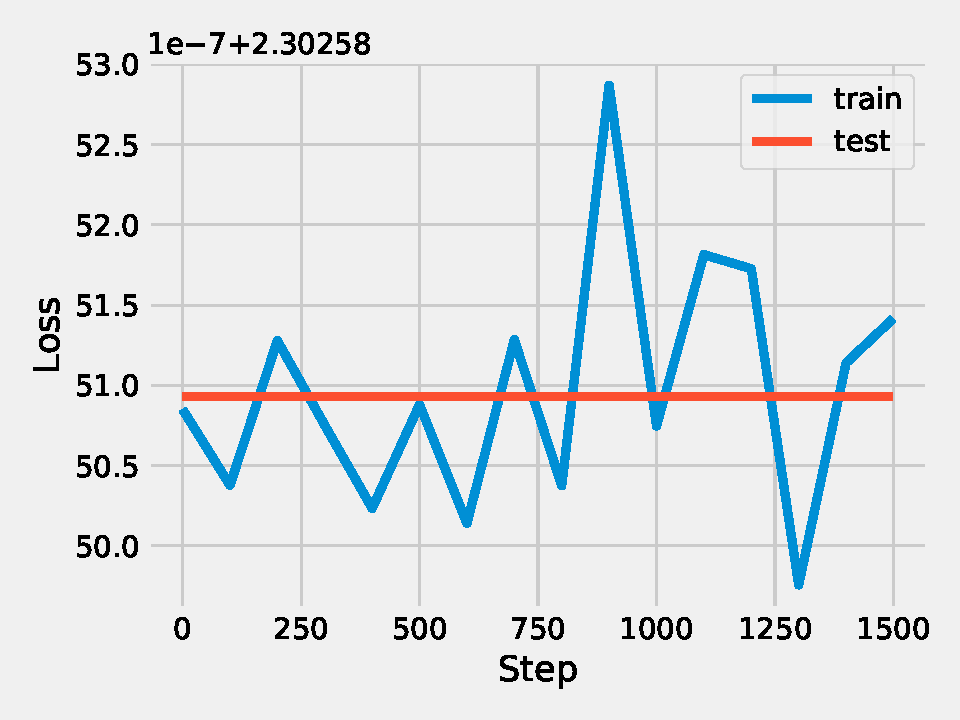
\includegraphics[width=\linewidth]{assignment_1/code/np_loss.pdf} &
    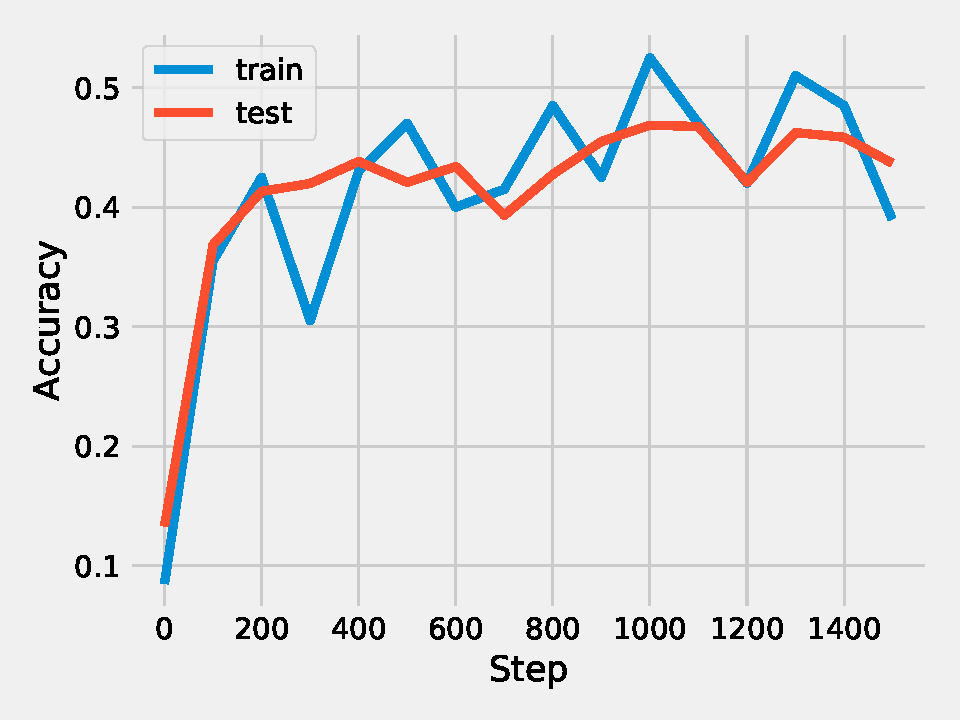
\includegraphics[width=\linewidth]{assignment_1/code/np_accuracy.pdf}
  \end{tabularx}
  \caption{\textbf{Left} the loss and \textbf{right} the accuracy during training of the NumPy MLP implementation.}
  \label{fig:numpy}
\end{figure}

\section{PyTorch MLP}
\begin{figure}
  \begin{tabularx}{\linewidth}{XX}
    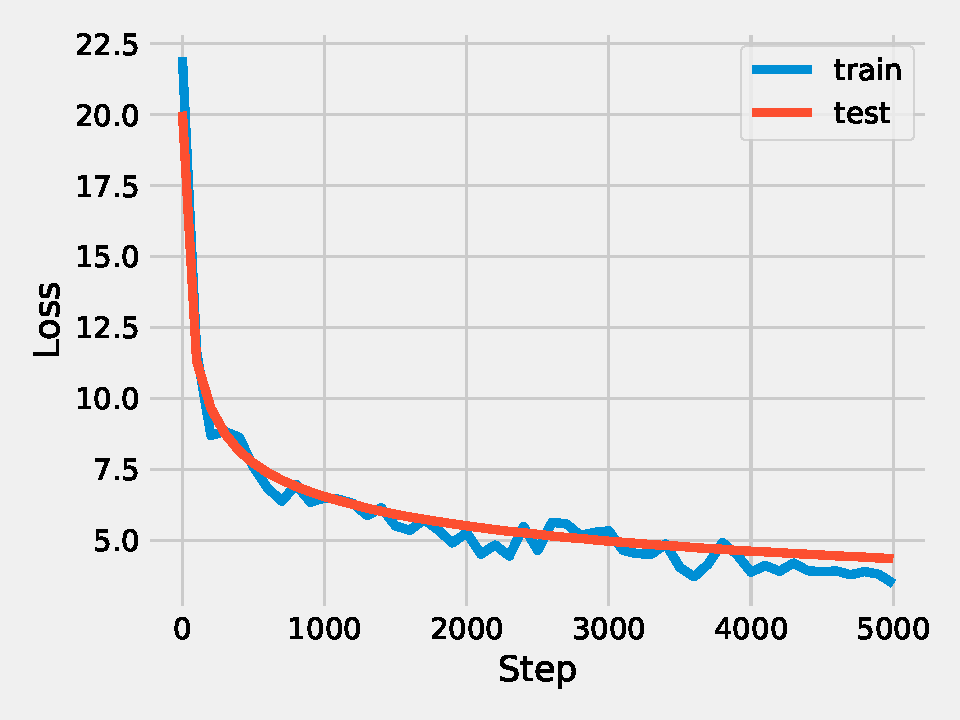
\includegraphics[width=\linewidth]{assignment_1/code/torch_loss.pdf} &
    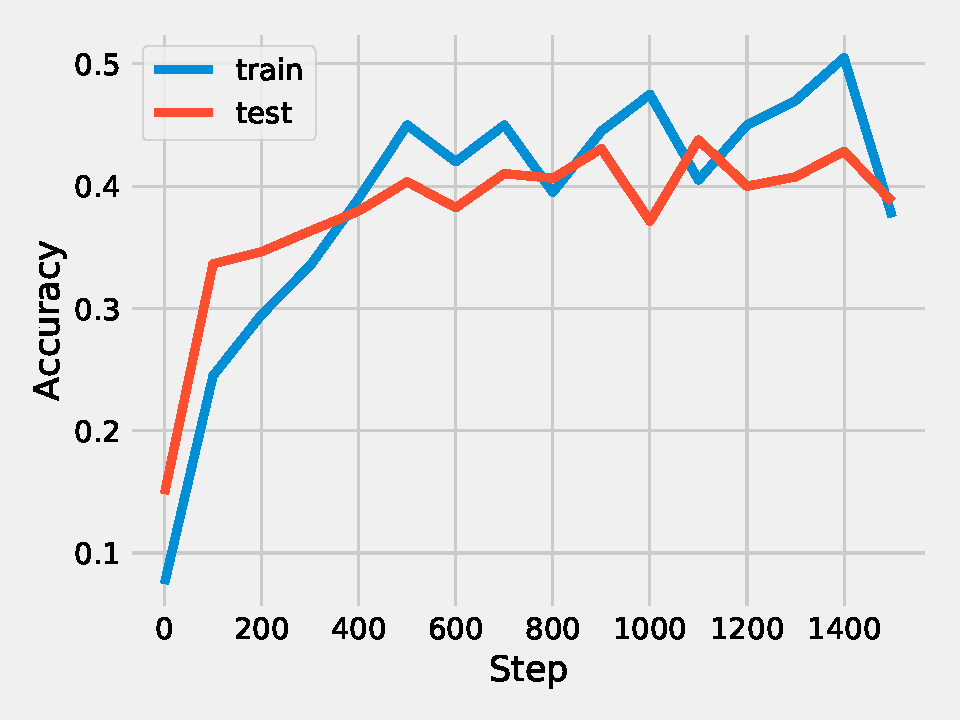
\includegraphics[width=\linewidth]{assignment_1/code/torch_accuracy.pdf}
  \end{tabularx}
  \caption{\textbf{Left} the loss and \textbf{right} the accuracy during training of the PyTorch MLP implementation.}
  \label{fig:pytorch_mlp}
\end{figure}

\end{document}
